%%%
%
% $Autor: Gargi Barve $
% $Date: 2026-04-27 12:00:00Z $
% $File: SARIMA.tex $
% $Version: 1 $
%
% Project: Time Series CPI Forecasting
%
%%%

\chapter{Seasonal AutoRegressive Integrated Moving Average (SARIMA)}
\label{ch:sarima}

\section{Description}
The Seasonal AutoRegressive Integrated Moving Average (SARIMA) model is a powerful extension to the classical ARIMA framework explicitly designed to capture and forecast time series data exhibiting periodic cycles. Standard ARIMA models rely on linear relationships with contiguous past observations to estimate trends, rendering them structurally blind to effects that repeat systematically over longer intervals (e.g., an observation $y_t$ being strongly correlated to the observation from a year ago $y_{t-12}$, rather than just yesterday $y_{t-1}$). SARIMA resolves this limitation by introducing the backshift operator $B$ at seasonal intervals. It formally constructs a composite model by mathematically multiplying a regular ARIMA polynomial by a seasonal ARIMA polynomial, adding dedicated parameters for seasonal autoregressive, seasonal moving average, and seasonal differencing terms. This multiplication of polynomials is mapped out in the flowchart in Figure~\ref{fig:sarima_tikz}.

\begin{figure}[htbp]
\centering
\resizebox{\linewidth}{!}{
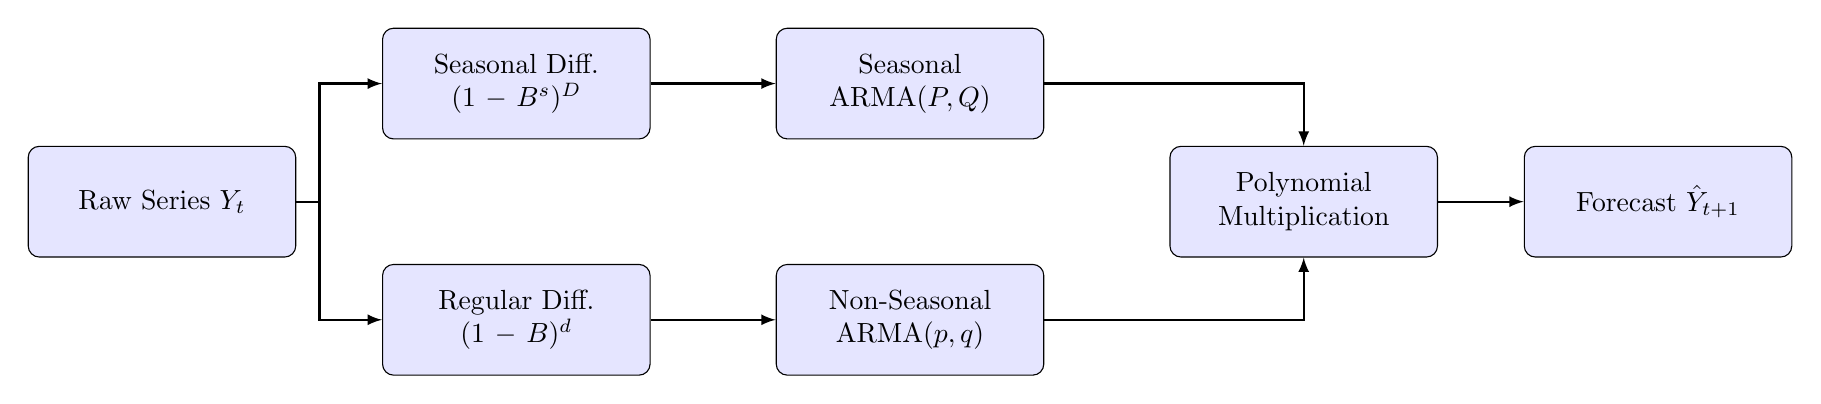
\begin{tikzpicture}[
    block/.style={rectangle, draw, fill=blue!10, text width=9em, text centered, rounded corners, minimum height=4em},
    line/.style={draw, -latex, thick}
]
    \node [block] (input) at (0,0) {Raw Series $Y_t$};
    
    \node [block] (sdiff) at (4.5,1.5) {Seasonal Diff. $(1-B^s)^D$};
    \node [block] (diff) at (4.5,-1.5) {Regular Diff. $(1-B)^d$};
    
    \node [block] (arma) at (9.5,-1.5) {Non-Seasonal ARMA($p,q$)};
    \node [block] (sarma) at (9.5,1.5) {Seasonal ARMA($P,Q$)};
    
    \node [block] (mult) at (14.5,0) {Polynomial Multiplication};
    \node [block] (output) at (19,0) {Forecast $\hat{Y}_{t+1}$};
    
    \draw [line] (input) -- (2,0) |- (sdiff);
    \draw [line] (2,0) |- (diff);
    
    \draw [line] (sdiff) -- (sarma);
    \draw [line] (diff) -- (arma);
    
    \draw [line] (sarma) -| (mult);
    \draw [line] (arma) -| (mult);
    \draw [line] (mult) -- (output);
\end{tikzpicture}

}
\caption{Architectural flowchart of a SARIMA model illustrating how the algorithm applies the backshift operator $B$ to construct and multiply non-seasonal and seasonal mathematical polynomials. Source: own diagram based on seasonal Box--Jenkins modeling \cite{Box2015,Hyndman2021}.}
\label{fig:sarima_tikz}
\end{figure}

\section{Applications}
SARIMA is the industry standard approach for modeling macroscopic and microscopic phenomena with pronounced, rigid seasonality. Application domains include forecasting airline passenger traffic, hotel bookings, energy consumption (where grid demand peaks annually in summer or winter), and agricultural retail sales. In macroeconomic planning, central banks rely on SARIMA to forecast series affected by annual tax cycles, quarterly corporate reporting, or periodic policy implementations.

\section{Relevance}
In this project, the underlying subject of study is the Consumer Price Index (CPI) of Germany. The CPI measures a "basket of goods" that inherently displays strong seasonal patterns due to predictable annual shifts in consumer behavior and market availability. Examples include winter heating oil demand spiking in November, summer vacation travel costs peaking in July, and bi-annual seasonal apparel releases. SARIMA is critical here; by mathematically isolating and explicitly modeling these cyclical variations via the seasonal parameter $s$, the algorithm mitigates seasonal "noise" that would otherwise corrupt a standard ARIMA model. This allows policymakers to more accurately predict "core" inflationary trends stripped of seasonal artifacts.

\section{Hyperparameters}
A SARIMA model is specified by a dual set of parameters, denoted as $(p, d, q) \times (P, D, Q)_s$:
\begin{itemize}
    \item \textbf{Non-Seasonal Parameters ($p, d, q$):} Define the standard AutoRegressive, Differencing, and Moving Average orders governing short-term, month-to-month dynamics.
    \item \textbf{Seasonal Parameters ($P, D, Q$):} Define the AutoRegressive, Differencing, and Moving Average orders applied specifically at the seasonal lags. For instance, $P=1$ means today's value is influenced by the value exactly one cycle ago.
    \item \textbf{Seasonal Period ($s$):} The length of the repeating seasonal cycle. For instance, in monthly data exhibiting annual seasonality, $s = 12$; in quarterly data, $s = 4$. Setting this value is crucial: if $s$ is too low (e.g., $s=1$), the model devolves into standard ARIMA and misses the macro-cycle. If $s$ is too high (e.g., $s=365$ for daily data), the polynomial complexity expands massively, requiring enormous amounts of historical data and computational power, often leading to over-fitting or failure to converge.
\end{itemize}

\section{Requirements}
SARIMA strictly requires that the underlying data-generating process is linear and that the seasonal period $s$ is consistent and known a priori. A fundamental requirement is sufficient historical data length: to properly estimate seasonal parameters and perform seasonal differencing, the dataset must contain at least two to three full seasonal cycles (e.g., 24-36 months of data for $s=12$). Similar to ARIMA, the series must achieve stationarity before parameter estimation. SARIMA achieves this via primary differencing ($y_t - y_{t-1}$) to eliminate trend, combined with seasonal differencing ($y_t - y_{t-s}$) to eliminate persistent cyclical patterns. Furthermore, the variance of the seasonal cycle must remain relatively constant; if the amplitude of the seasons grows over time, a log transformation is required beforehand.

\section{Input}
The algorithm requires a univariate, continuously indexed sequence of observations. In Python, this is instantiated as a \texttt{pandas.Series} possessing a strict chronological index. Accurate metadata regarding the frequency of the observations must be explicitly provided, as the model relies on this to calculate the $s$ parameter mathematically.

\section{Output}
SARIMA outputs an extrapolated series of predicted values extending into the future. Due to its structural mathematical properties, it uniquely recalculates both the short-term trend and the periodic peaks/troughs simultaneously for every future step. It also returns standard errors and likelihood metrics (such as AIC/BIC), which are utilized to generate probabilistic confidence intervals quantifying the bounds of the forecast.

\section{Example with a program}
The \texttt{statsmodels} library in Python implements SARIMA via the robust \texttt{SARIMAX} class. (The 'X' denotes support for eXogenous variables, which can be ignored by passing solely the endogenous series):

\begin{Python}[caption={SARIMA Implementation using Statsmodels}, label={lst:sarima_python}]
import pandas as pd
from statsmodels.tsa.statespace.sarimax import SARIMAX

# 'cpi_series' is a pandas Series with a monthly DatetimeIndex
# In this hypothetical, we have 3 years of data (36 observations)
cpi_series = pd.Series([105.1, 105.4, 105.8, 106.2, 106.5])

# Initialize a SARIMA model:
# Short-term (non-seasonal) dynamics: (1,1,1)
# Annual seasonal dynamics: P=1, D=1, Q=1 with a 12-month cycle (s=12)
model = SARIMAX(endog=cpi_series, 
                order=(1, 1, 1), 
                seasonal_order=(1, 1, 1, 12),
                enforce_stationarity=False,
                enforce_invertibility=False)

# Fit the model via Maximum Likelihood Estimation
fitted_model = model.fit(disp=False)

# Forecast the next 12 periods and retrieve confidence intervals
forecast_result = fitted_model.get_forecast(steps=12)
predictions = forecast_result.predicted_mean
conf_ints = forecast_result.conf_int(alpha=0.05) # 95% Confidence Bounds

print(predictions)
\end{Python}

\section{Further Reading}
\begin{itemize}
    \item Box, G. E. P., Jenkins, G. M., Reinsel, G. C., \& Ljung, G. M. (2015). \textit{Time Series Analysis: Forecasting and Control} (5th ed.). John Wiley \& Sons. (The definitive text on seasonal Box-Jenkins models).
    \item Hyndman, R. J., \& Athanasopoulos, G. (2018). \textit{Forecasting: Principles and Practice} (2nd ed.). OTexts. Available at \url{https://otexts.com/fpp2/seasonal-arima.html}. \cite{Hyndman2018}
\end{itemize}
